\documentclass[tikz,border=4pt]{standalone}
\usepackage{pgfplots}
\pgfplotsset{compat=1.18}
\usepgfplotslibrary{groupplots}
\begin{document}
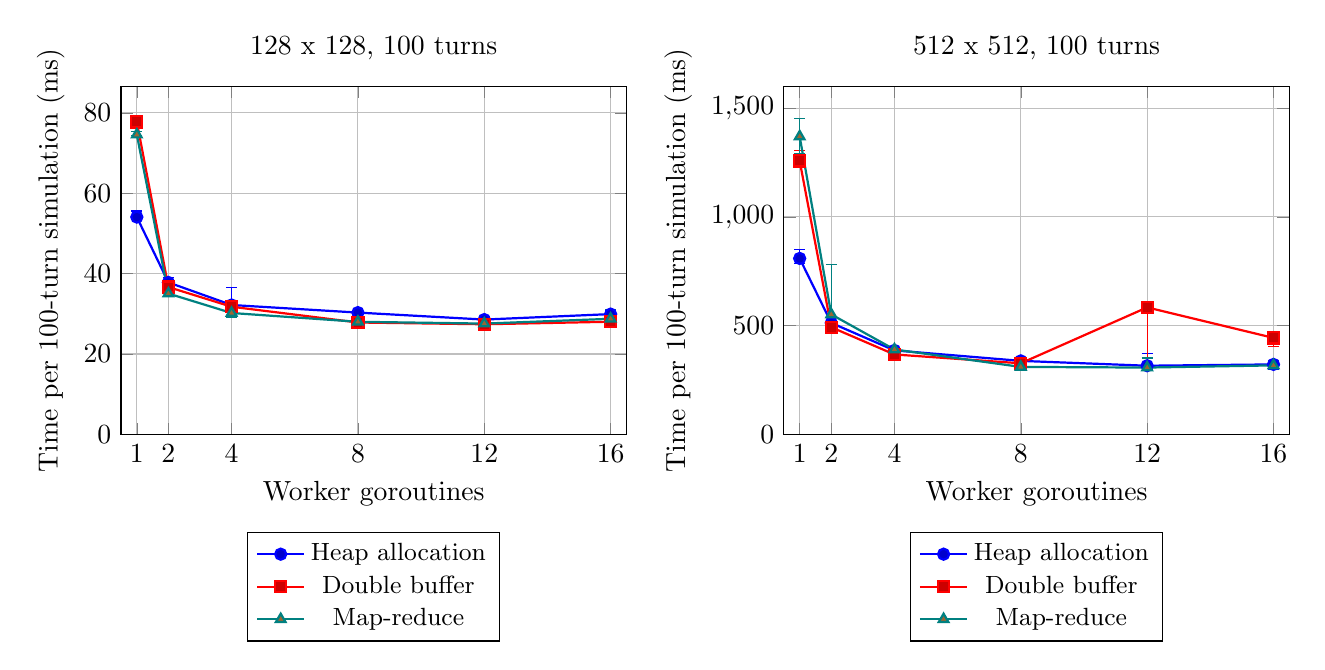
\begin{tikzpicture}
\begin{groupplot}[group style={group size=2 by 1,horizontal sep=20mm},
width=8cm,height=6cm,xlabel={Worker goroutines},
ylabel={Time per 100-turn simulation (ms)},
xtick={1,2,4,8,12,16},xmin=0.5,xmax=16.5,ymin=0,grid=major,
legend style={font=\small,at={(0.5,-0.28)},anchor=north}]
\nextgroupplot[title={128 x 128, 100 turns}]
\addplot+[color=blue,mark=*,thick,error bars/.cd,y dir=both,y explicit] coordinates {(1,54.082156) += (0,1.514717) -= (0,0.153289) (2,37.817423) += (0,1.181897) -= (0,0.382796) (4,32.202175) += (0,4.396878) -= (0,0.631652) (8,30.313198) += (0,0.534064) -= (0,0.285492) (12,28.577697) += (0,0.645054) -= (0,0.207145) (16,29.940383) += (0,0.885241) -= (0,0.978699)};
\addlegendentry{Heap allocation}
\addplot+[color=red,mark=square*,thick,error bars/.cd,y dir=both,y explicit] coordinates {(1,77.769082) += (0,0.934212) -= (0,0.660025) (2,36.665534) += (0,0.571703) -= (0,0.190597) (4,31.771743) += (0,1.560652) -= (0,0.250883) (8,27.849576) += (0,1.738475) -= (0,0.782987) (12,27.406587) += (0,1.156128) -= (0,0.402000) (16,28.038509) += (0,1.503738) -= (0,0.496003)};
\addlegendentry{Double buffer}
\addplot+[color=teal,mark=triangle*,thick,error bars/.cd,y dir=both,y explicit] coordinates {(1,74.597434) += (0,0.777393) -= (0,0.205202) (2,35.047575) += (0,1.469005) -= (0,0.380238) (4,30.213155) += (0,0.823106) -= (0,1.049919) (8,28.022981) += (0,1.071761) -= (0,0.125500) (12,27.576712) += (0,1.261258) -= (0,0.280781) (16,28.771198) += (0,2.397325) -= (0,0.110100)};
\addlegendentry{Map-reduce}
\nextgroupplot[title={512 x 512, 100 turns}]
\addplot+[color=blue,mark=*,thick,error bars/.cd,y dir=both,y explicit] coordinates {(1,809.032218) += (0,40.071550) -= (0,21.252070) (2,512.576745) += (0,28.478108) -= (0,5.788505) (4,386.231767) += (0,4.250151) -= (0,13.630218) (8,338.053009) += (0,15.593936) -= (0,17.153727) (12,315.740071) += (0,56.428863) -= (0,17.202020) (16,321.804629) += (0,18.685127) -= (0,21.866603)};
\addlegendentry{Heap allocation}
\addplot+[color=red,mark=square*,thick,error bars/.cd,y dir=both,y explicit] coordinates {(1,1257.428461) += (0,46.369682) -= (0,3.860911) (2,492.693235) += (0,1.407158) -= (0,2.559963) (4,367.485138) += (0,6.608340) -= (0,3.329201) (8,326.902948) += (0,6.738007) -= (0,8.519483) (12,583.937138) += (0,25.967888) -= (0,271.108592) (16,443.703939) += (0,1.526141) -= (0,39.831378)};
\addlegendentry{Double buffer}
\addplot+[color=teal,mark=triangle*,thick,error bars/.cd,y dir=both,y explicit] coordinates {(1,1369.583975) += (0,84.531125) -= (0,79.397212) (2,551.650077) += (0,231.084315) -= (0,38.443647) (4,390.367926) += (0,9.051525) -= (0,31.339124) (8,310.286925) += (0,24.927749) -= (0,3.861770) (12,307.357640) += (0,43.783080) -= (0,1.027182) (16,317.336201) += (0,20.900251) -= (0,13.973511)};
\addlegendentry{Map-reduce}
\end{groupplot}
\end{tikzpicture}
\end{document}
